%%%%%%%%%%%%%%%%%%%%%%%%%%%%%%%%%%%%%%%%%
% University Assignment Title Page 
% LaTeX Template
% Version 1.0 (27/12/12)
%
% This template has been downloaded from:
% http://www.LaTeXTemplates.com
%
% Original author:
% WikiBooks (http://en.wikibooks.org/wiki/LaTeX/Title_Creation)
%
% License:
% CC BY-NC-SA 3.0 (http://creativecommons.org/licenses/by-nc-sa/3.0/)
%
%%%%%%%%%%%%%%%%%%%%%%%%%%%%%%%%%%%%%%%%%
%\title{Title page with logo}
%----------------------------------------------------------------------------------------
%	PACKAGES AND OTHER DOCUMENT CONFIGURATIONS
%----------------------------------------------------------------------------------------

\documentclass[12pt]{article}
\usepackage[english]{babel}
\usepackage[utf8x]{inputenc}
\usepackage{natbib}
\usepackage{amsmath}
\usepackage[colorinlistoftodos]{todonotes}
\usepackage{listings}
\usepackage{color}
\usepackage{tabu}
\tabulinesep=1.2mm
\usepackage[explicit]{titlesec}
\usepackage{url}
\usepackage{subfig}
\usepackage{graphicx}
\usepackage{grffile}
\usepackage{mwe}
\usepackage[section]{placeins}

\begin{document}

\begin{titlepage}

\newcommand{\HRule}{\rule{\linewidth}{0.5mm}} % Defines a new command for the horizontal lines, change thickness here

\center % Center everything on the page
 
%----------------------------------------------------------------------------------------
%	HEADING SECTIONS
%----------------------------------------------------------------------------------------

\textsc{\LARGE University of St Andrews}\\[1.5cm] % Name of your university/college
\textsc{\Large CS4204 Coursework 1}\\[0.5cm] % Major heading such as course name
\textsc{\large }\\[0.5cm] % Minor heading such as course title

%----------------------------------------------------------------------------------------
%	TITLE SECTION
%----------------------------------------------------------------------------------------

\HRule \\[0.4cm]
{ \huge \bfseries Parallel Patterns}\\[0.4cm] % Title of your document
\HRule \\[1.5cm]
 
%----------------------------------------------------------------------------------------
%	AUTHOR SECTION
%----------------------------------------------------------------------------------------


\Large \emph{Author:}\\
 \textsc{150008022}\\[3cm] % Your name

%----------------------------------------------------------------------------------------
%	DATE SECTION
%----------------------------------------------------------------------------------------

{\large \today}\\[2cm] % Date, change the \today to a set date if you want to be precise

%----------------------------------------------------------------------------------------
%	LOGO SECTION
%---------------------------------------------------------------------------------------


\includegraphics[width = 3.1cm]{images/standrewslogo.png}
 
%----------------------------------------------------------------------------------------

\vfill % Fill the rest of the page with whitespace

\end{titlepage}

\section*{Goal}

To implement and evaluate a library for parallelising C programs, using PThreads, locks, and queues. 

\section{Blocking Queue}

The implementation of parallel task handlers would have to accumulate their outputs and buffer their inputs in a thread safe way, and so a blocking queue was necessary. \lstinline{queue.h} provides an interface for a queue to be used by other components, and \lstinline{queue.c} provides an implementation.

The queue is a linked list structure, where each node in the list has a reference to the element next in line. The queue structure tracks the last in line for adding new nodes, and the first in line for removing nodes. A conditional variable is used to notify threads waiting to add or remove elements that the size of the queue has changed, and a normal mutex is used to ensure that only one node is able to perform the addition or removal at a time. Figure \ref{fig:queue} shows a queue struct with a series of node structs.

For convenience, the destroyer function for the queue also takes the destroyer function for its elements as a parameter so that it can be assumed that destroying a queue will free all memory that it is responsible for.

\begin{figure}[!ht]
	\centering 
	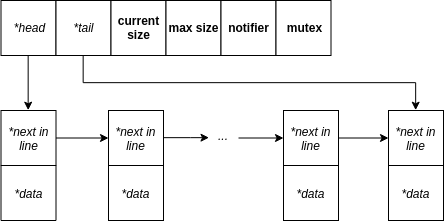
\includegraphics[width=0.8\linewidth]{images/queue}
	\caption{Queue structure, showing head and tail pointers, and each member of queue referencing the next.}
	\label{fig:queue}
\end{figure}

\section{Pipeline} 

The pipeline pattern is where a series of functions are applied to some input. Often the analogy of a conveyor belt is used, as inputs can flow continuously and functions can be applied simultaneously to inputs that are at differenet stages of the pipeline.

Figure \ref{fig:pipe} shows how an atomic pipeline was implemented for this submission. An array of functions are submitted on creation of the pipeline, along with the number of worker threads that should run for each stage in the pipeline. The pipeline interface allows for inputs to be added to a queue, where they will wait to be processed, and for outputs to be polled from the outgoing queue. 

\begin{figure}[!ht]
	\centering 
	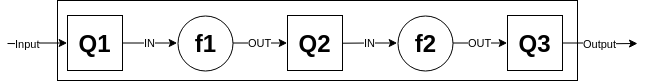
\includegraphics[width=\linewidth]{images/pipe}
	\caption{Pipeline abstraction, where Q signifies a blocking queue, and f signifigies a function being applied.}
	\label{fig:pipe}
\end{figure}

The pipeline was defined to consist of a series of steps which would be managed by a thread. The thread for step $i$ would poll queue $Q_i$ for an input $x$ to process, compute $f(x)$, then add the output to queue $Q_{i+1}$. $Q_0$ and $Q_{n+1}$ are the input and output queues made accessible by the pipeline interface, where $n$ is the number of functions in the pipeline.

\begin{figure}[!ht]
	\centering 
	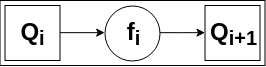
\includegraphics[width=0.45\linewidth]{images/step}
	\caption{Step of pipeline.}
	\label{fig:step}
\end{figure}

\section{Parallel Farm}

The parallel farm pattern involves a pool of worker threads that remain idle until assigned a task by a coordinator. Once a worker thread completes its task, it then returns to being idle until a new task is assigned. Parallel farms are useful as they avoid the overhead involved .

\begin{figure}[!ht]
	\centering 
	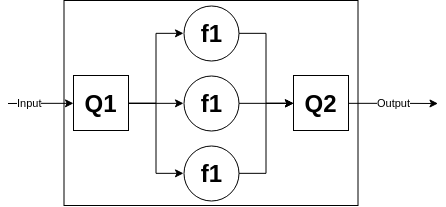
\includegraphics[width=0.8\linewidth]{images/farm}
	\caption{Farm abstraction}
	\label{fig:farm}
\end{figure}

\section*{Conclusion}

%\bibliographystyle{unsrt}
%\bibliography{mybib}

\end{document}
